
\subsubsection{Dostava paketa}

	\begin{itemize}
		\item{Kratak opis:} 
		\begin{itemize}
			\item{Dostavljač dobija informacije o paketu od sistema i dostavlja paket korisniku.}
		\end{itemize}
		
		\item{Učesnici:} 
		\begin{itemize}
			\item{Dostavljač, korisnik}
		\end{itemize}		
		
		\item{Preduslovi:}
		\begin{itemize}
			\item{Dostavljač je prijavljen na sistem i ima nedostavljenih paketa. }
			\item{Klijent je poručio paket.}
		\end{itemize}		

		\item{Postuslovi:}
		\begin{itemize}
			\item{Korisnik dobija svoj paket sa namirnicama.}
		\end{itemize}		
		
		\item{Osnovni tok:}
		\begin{enumerate}
			\item{Dostavljač dobija obaveštenje od sistema da ima nedostavljenih paketa.}
			\item{Dostavljač dolazi do magacina gde su smešteni paketi.}
			\item{Dostavljač očitava identifikacioni broj paketa pomoću sistema i dobija informacije o porudžbini.}
			\item{Dostavljač dolazi do destinacije korisnika u predviđenom periodu.}
			\item{Korisnik preuzima svoj paket.}
			\item{Dostavljač beleži da je uspešno izvršio dostavu.}
			
			
			\textit{Koraci 2-6 se ponavljaju sve dok ima nedostavljenih paketa.}
		\end{enumerate}
		
		\item{Alternativni tokovi:}
			\begin{enumerate}
				\item[4.a] Ukoliko dostavljač proceni da će kasniti, obaveštava korisnika pomoću sistema.
				\item[5.a] Ukoliko korisnik nije na naznačenoj adresi, dostavljač ostavlja paket ispred ulaza. Slučaj upotrebe se nastavlja od koraka 6.%Sistem obaveštava korisnika da dostavljač nije uspeo da dostavi paket i traži od korisnika da potvrdi svoju adresu. Ako je korisnik promenio adresu, sistem ga navodi na opciju ažuriranja naloga.  
			\end{enumerate}
		\item{Dodatne informacije:}
			\begin{itemize}
				\item{Spisak nedostavljenih paketa je sortiran rastuće po vremenu dostave.}
			\end{itemize}
	\end{itemize}
	
\begin{figure}[H]
	\begin{center}
		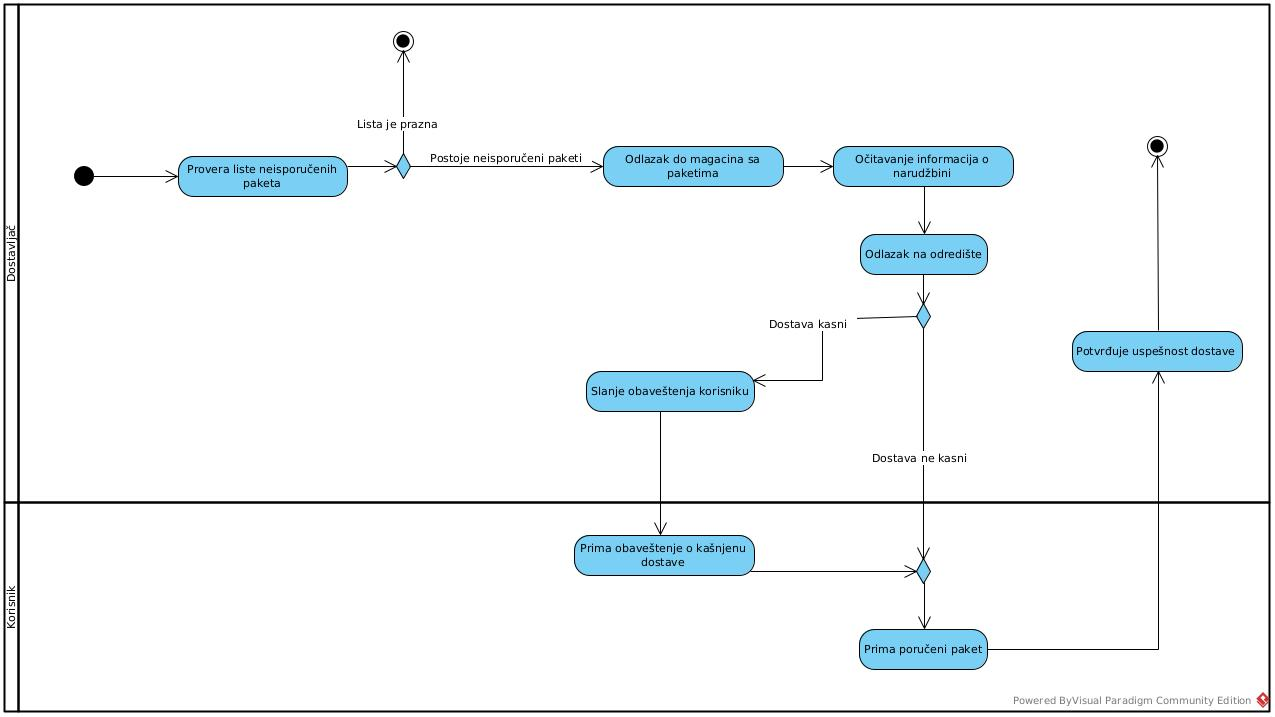
\includegraphics[width=1\textwidth]{activity_package_delivery}
	\end{center}
	\caption{Dijagram aktivnosti dostave paketa}
%	\label{fig:UCPackageDelivery}
\end{figure}	
